\documentclass[UTF8]{ctexart}
\usepackage{geometry}
\usepackage{listings}
\usepackage{xcolor}
\usepackage{graphicx}
\usepackage{amsmath}
\usepackage{float}
\usepackage{hyperref}
\usepackage{algorithm}
\usepackage{algpseudocode} % algorithmicx 的一部分
\geometry{a4paper, left=2.5cm, right=2.5cm, top=2.5cm, bottom=2.5cm}

\title{\textbf{Computing the Dot Product of TwoVector}}
\author{
    Author: 李语尚 12412308
    \newline
    Date: \today
}
\date{}

\lstset{
    basicstyle=\ttfamily\small,
    keywordstyle=\color{blue},
    commentstyle=\color{gray},
    stringstyle=\color{red},
    frame=single,
    breaklines=true,
    numbers=left,
    numberstyle=\tiny\color{gray},
    language=C
}

\begin{document}

\maketitle
\tableofcontents
\newpage

\section{前言}
\subsection{简介}
这学期的ada课，通常助教要求java的运行时间在2s以内，cpp的运行时间在1s以内，也就是说大家预设了java的运行时间是c的两倍，上个学期的dsaa课上，我们通常会根据题目要求的时间以及运行时间来大体判断这道题的时间复杂度被限制在多少。不管是java还是cpp，好像运行时间的要求又是一样的了。
这似乎非常矛盾，到底java的时间要求比cpp长还是一样，并且这两种语言为什么会有这些差异?这些差异来自于哪里?
这个project引出了许多问题，也是我之前遇到过，但是没有详细思考过的。
这个project将通过计算不同size的向量点积，聚焦于c与java编译、执行的不同之处，分析这两种语言运行时间的不同的差异来自于哪里。作为一个写了很久的java选手，我将进一步研究不同jdk以及有无多线程这些变量对于java运行时间的影响。
\subsection{测试任务}
统一测试任务为数组点乘：
\[
\text{sum} = \sum_{i=0}^{N-1} a_i b_i
\]
该任务理论复杂度为 $O(N)$，因此不同实现的性能差异主要来自常数因子、编译优化和运行时策略。

\subsection{对比维度}
本报告包含 5 组核心对比：
\begin{itemize}
    \item C 无优化 vs JDK 17 无优化
    \item C 无优化 vs C \texttt{-O3}
    \item JDK 17 vs JDK 26（无额外优化）
    \item JDK 26 无优化 vs JDK 26 优化方案
    \item C \texttt{-O3} vs JDK 26
\end{itemize}
\section{测试内容}
\subsection{数据一致性}
在离散数学课上学过 LCG算法，它对应着 C 语言标准库中的 \texttt{rand()} 函数。
其生成伪随机数的核心递推公式为：
\[
N_{j+1} \equiv (A \times N_{j} + B) \pmod{M}
\]

不难发现，由于通过线性同余方法构建的伪随机数生成器的内部状态很容易被其输出逆向推演，其低位通常存在极其明显的周期性规律。经过资料查询，现在企业级应用都在使用PCG算法。相比传统的 LCG，PCG结合了 64 位 LCG 状态推进和 Xorshift 输出置换机制，能在极低计算开销下提供极长周期（$2^{64}$），并彻底消除低位规律对 CPU 缓存和分支预测等底层微架构优化所带来的干扰。

因此，为避免“数据生成”阶段成为计算瓶颈或引入测试偏差，C 端不再使用传统的 \texttt{rand()}，而是使用轻量且统计特性优良的 PCG32 伪随机数算法，更适合海量数据的高精度性能基准测试。其核心代码如下：

\begin{lstlisting}
// 1. 状态推进: 64-bit LCG
rng.state = oldstate * 6364136223846793005ULL + (rng.inc | 1);

// 2. 输出置换: XSH-RR
uint32_t xorshifted = ((oldstate >> 18u) ^ oldstate) >> 27u;
uint32_t rot = oldstate >> 59u;
return (xorshifted >> rot) | (xorshifted << ((-rot) & 31));
\end{lstlisting}

\subsection{C 语言高精度性能测速机制}
为了确保 C 语言基准测试结果的绝对严谨性，排除系统或外围操作的干扰，我们在测速代码的实现中采用了严格的控制变量机制。具体体现在以下两点核心优化：

\begin{itemize}
    \item \textbf{分离数据生成与核心计算}：在很多不严谨的基准测试中，往往会将内存分配（\texttt{malloc}）或随机数生成的时间算入总时长。而在我们的 C 测试程序中，动态内存的申请以及由 PCG32 生成巨量随机数据的过程全部被安排在计时器开始之前，确保庞大的 PRNG（伪随机数生成器）位运算耗时绝对不会污染最终点乘算术的时间数据。
    \item \textbf{精准收缩测速边界与避免时钟倾斜}：为了达到真实物理时间（Wall-clock time）的纳秒级精度，我们选用了 Linux 环境下的 \texttt{clock\_gettime(CLOCK\_MONOTONIC, \&start)}，而非 C 标准库的 \texttt{clock()} 函数。
    \begin{itemize}
        \item \textbf{\texttt{clock()} 的致命缺陷}：\texttt{clock()} 测量的是“CPU 占用时间（CPU time）”，即所有线程在 CPU 上执行时间的总和。如果在多线程跑基准测试，\texttt{clock()} 会把 1 秒钟的真实流逝时间放大为 $1 \times N_{threads}$ 秒，导致测速结果极其失真。其次，部分系统的 \texttt{clock()} 精度仅能达到微秒甚至毫秒级。
        \item \textbf{\texttt{CLOCK\_MONOTONIC} 的优势}：它是一把不受系统闰秒调整、时间同步（NTP）干预的“单调物理绝对秒表”。该计时函数被精准且极其贴身地卡在了核心的核心 \texttt{for} 循环两端：只有在真正进入点乘累加操作时才启动计时，并在循环结束的瞬间立即终止。
    \end{itemize}
\end{itemize}

代码结构示例如下：
\begin{lstlisting}[language=C]
// 【机制 1】提前生成数据，内存分配及随机数生成均不计入测速时间
for (int i = 0; i < size; i++) {
    a[i] = generate_int();
    b[i] = generate_int();
}

long long sum = 0;
TimeSpec start, end;

// 【机制 2】卡紧边界，只对真实极简的计算循环进行纯粹测速
clock_gettime(CLOCK_MONOTONIC, &start);
for (int i = 0; i < size; i++) {
    sum += (long long)a[i] * b[i];
}
clock_gettime(CLOCK_MONOTONIC, &end);
\end{lstlisting}

这种极致纯粹、只有取指与乘加运算的紧凑循环结构，不仅保证了秒表数据的物理意义纯粹性，也在客观上极大地迎合了现代 C 编译器（如 GCC \texttt{-O3} 优化）。它允许编译器毫无顾忌地将标量操作映射至 CPU 的 AVX 向量寄存器，为探究处理器的理论算力极限铺平了道路。

拥有了高质量的随机数和极度纯粹的测速机制，我们就可以正式开始对不同类型的数据以及不同平台的性能进行极限压测。

\section{结果}
\subsection{预备工作}
为保证性能测试的相对公平性，所有实验均在同一台物理设备的隔离环境下完成，并且进行连续测试，争取达到在电脑状态基本不变的情况，并且取五次实验的平均值，避免偶然性，硬件与系统配置详情如下：
\begin{itemize}
    \item \textbf{CPU}：AMD Ryzen 9 7940HX (2.40 GHz)
    \item \textbf{物理内存}：16.0 GB
    \item \textbf{宿主操作系统}：Windows 64 位
    \item \textbf{C 语言测试环境}：WSL 环境下的 GCC 编译器
    \item \textbf{Java 测试环境}：IntelliJ IDEA，分别使用 JDK 17 和 JDK 26 版本
\end{itemize}
我们一共有int，float,double,short,signed char五种类型进行实验
求点积的伪代码如下：
\begin{lstlisting}
function dot_product_basic(A, B, N):
    sum = 0
    for i from 0 to N - 1:
        sum = sum + A[i] * B[i]
    return sum
\end{lstlisting}
\subsection{对比1: C 无优化 vs JDK 17 无优化}
\begin{figure}[H]
    \centering
    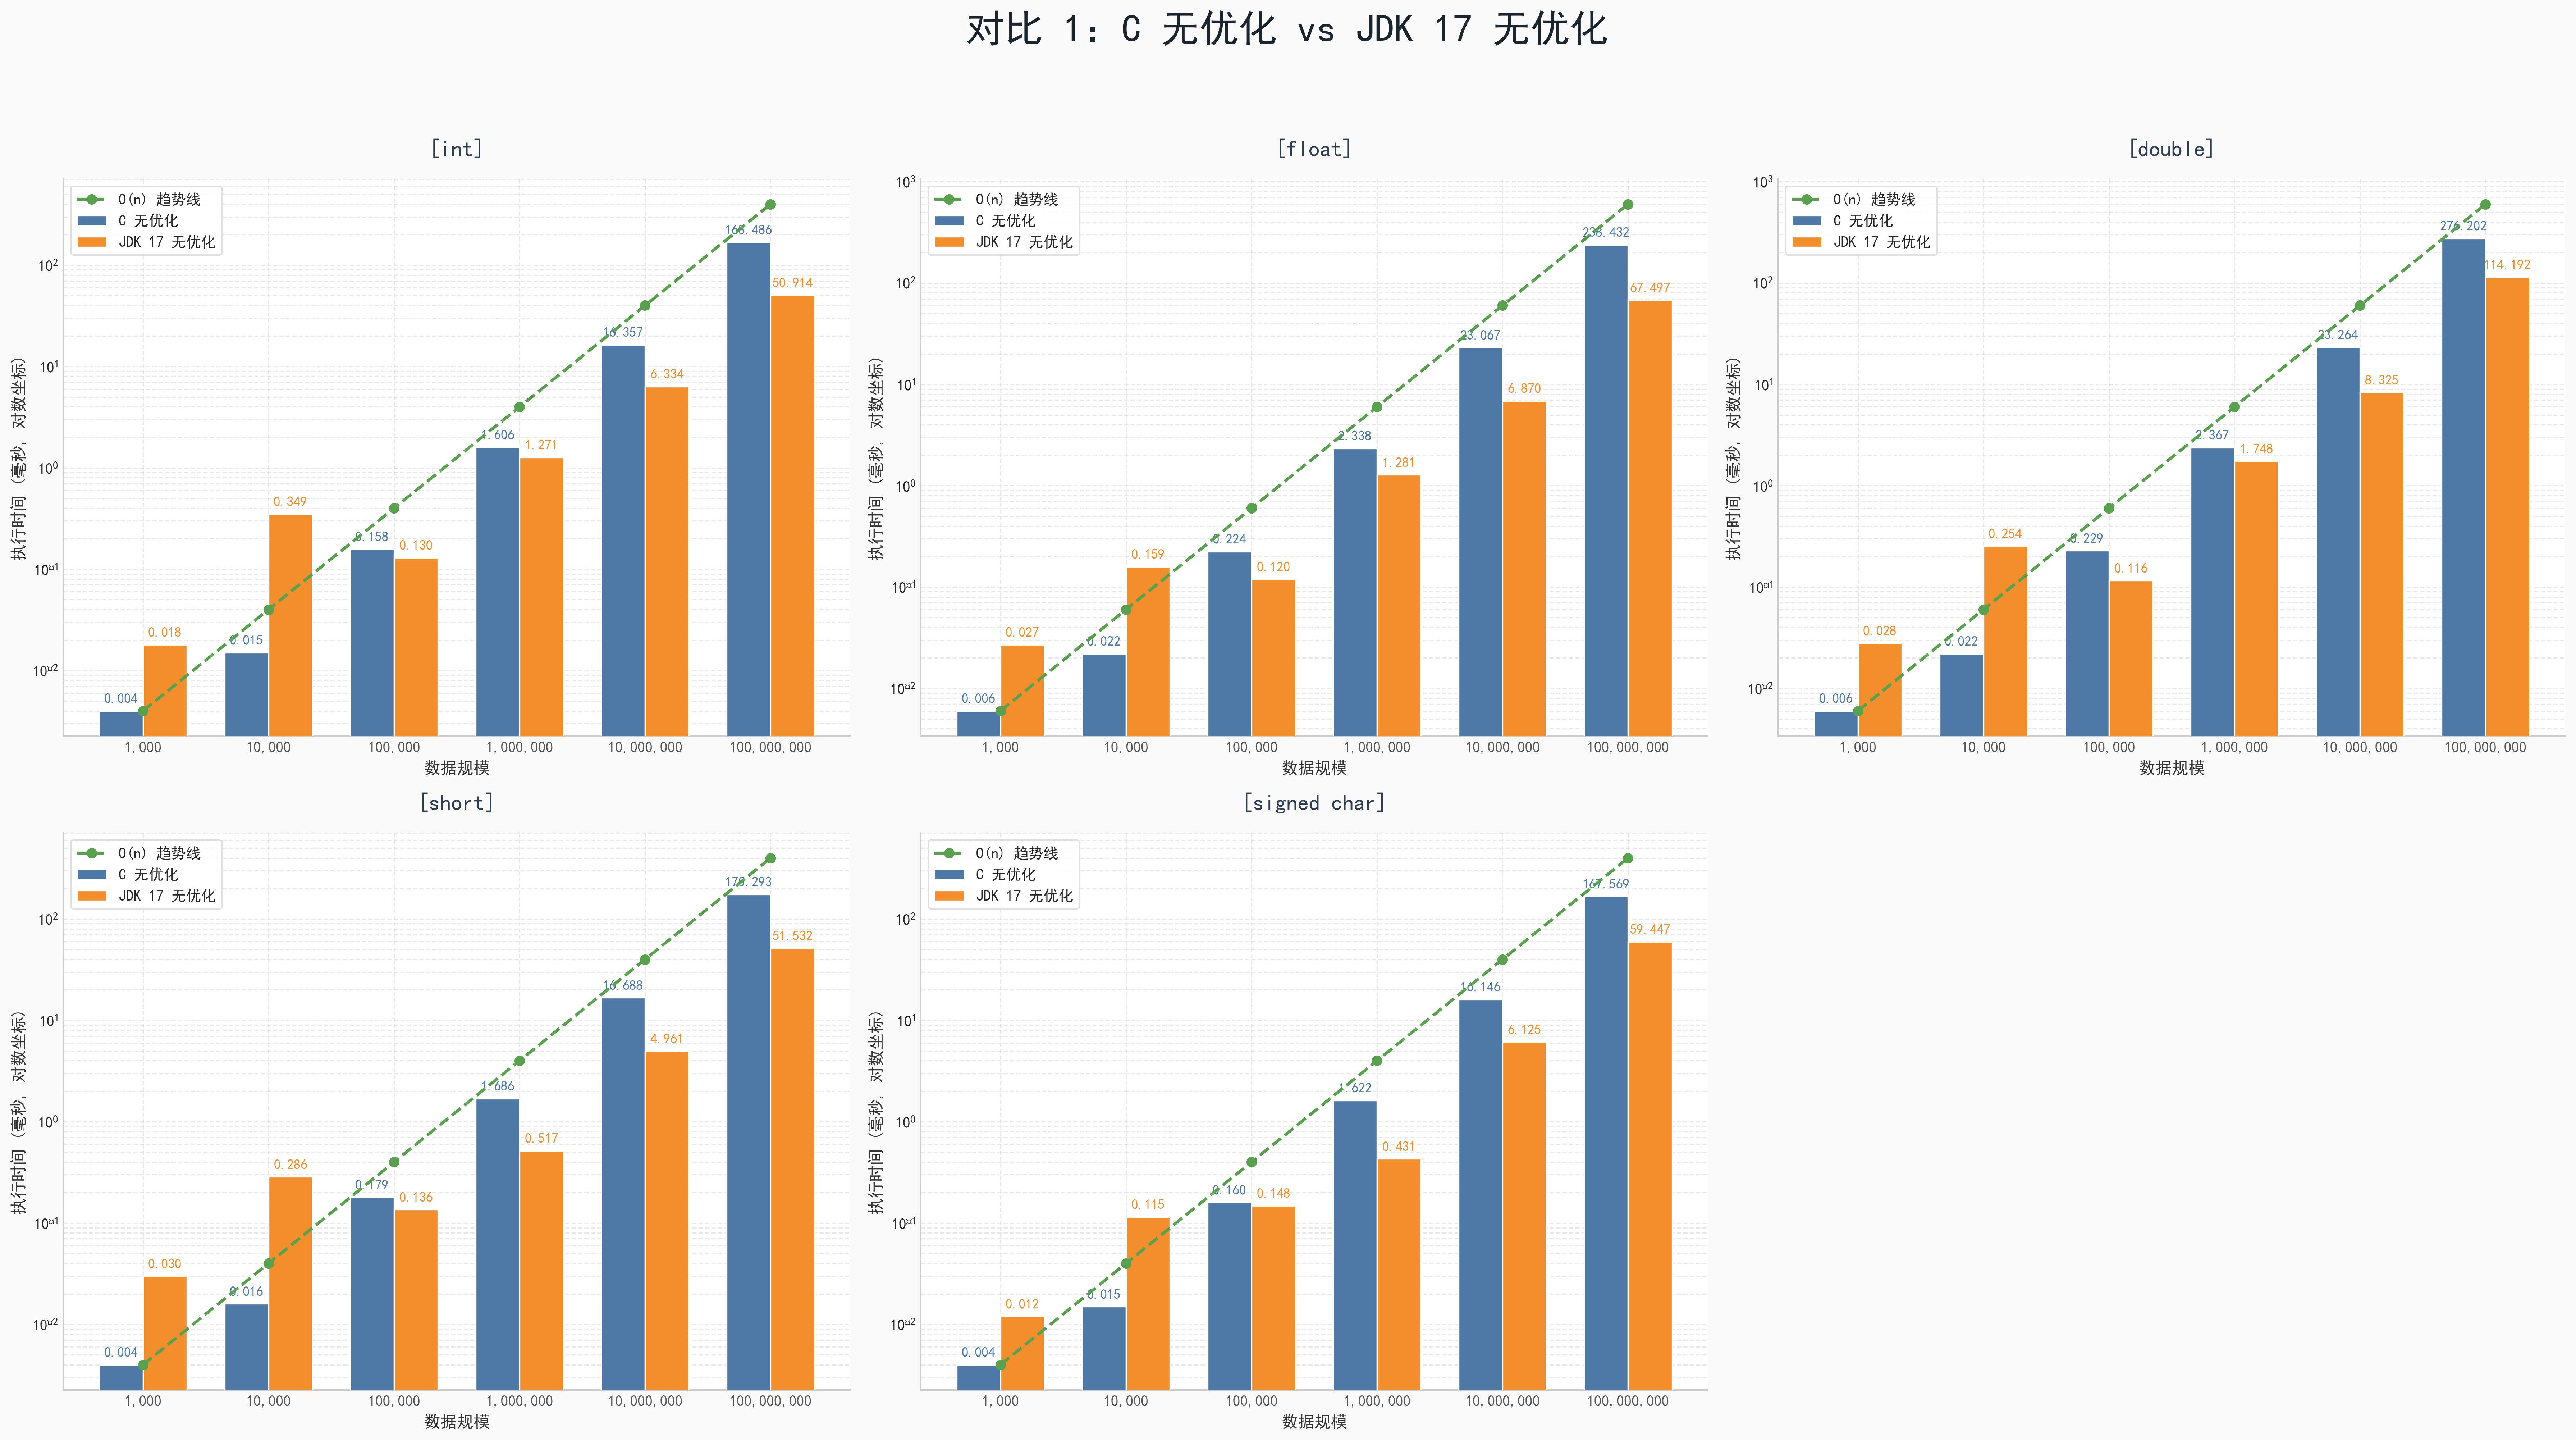
\includegraphics[width=0.92\textwidth]{1_c_vs_jdk17_noopt_ALL.png}
    \caption{C 无优化 vs JDK 17 无优化}
\end{figure}
我们能清楚的发现，C语言随着size增长，运行时间基本是很完美的线性增长，但是对于java来说，它的增长规律看似是线性的，但是在10k到100k这个数据规模的时候，似乎有一些反常，100k反而总时间比10k短，而且我们能发现java在数据规模小的时候运行时间是比较长的，之后增长速度变快，后面运行时间比c语言反而慢了许多。由于对数坐标的原因我们似乎看不出来这个差异，但是从数据来看，c语言的运行速度是java的好几倍。之后我们会进行分析。


\subsection{对比 2: C 无优化 vs C \texttt{-O3}}
\begin{figure}[H]
    \centering
    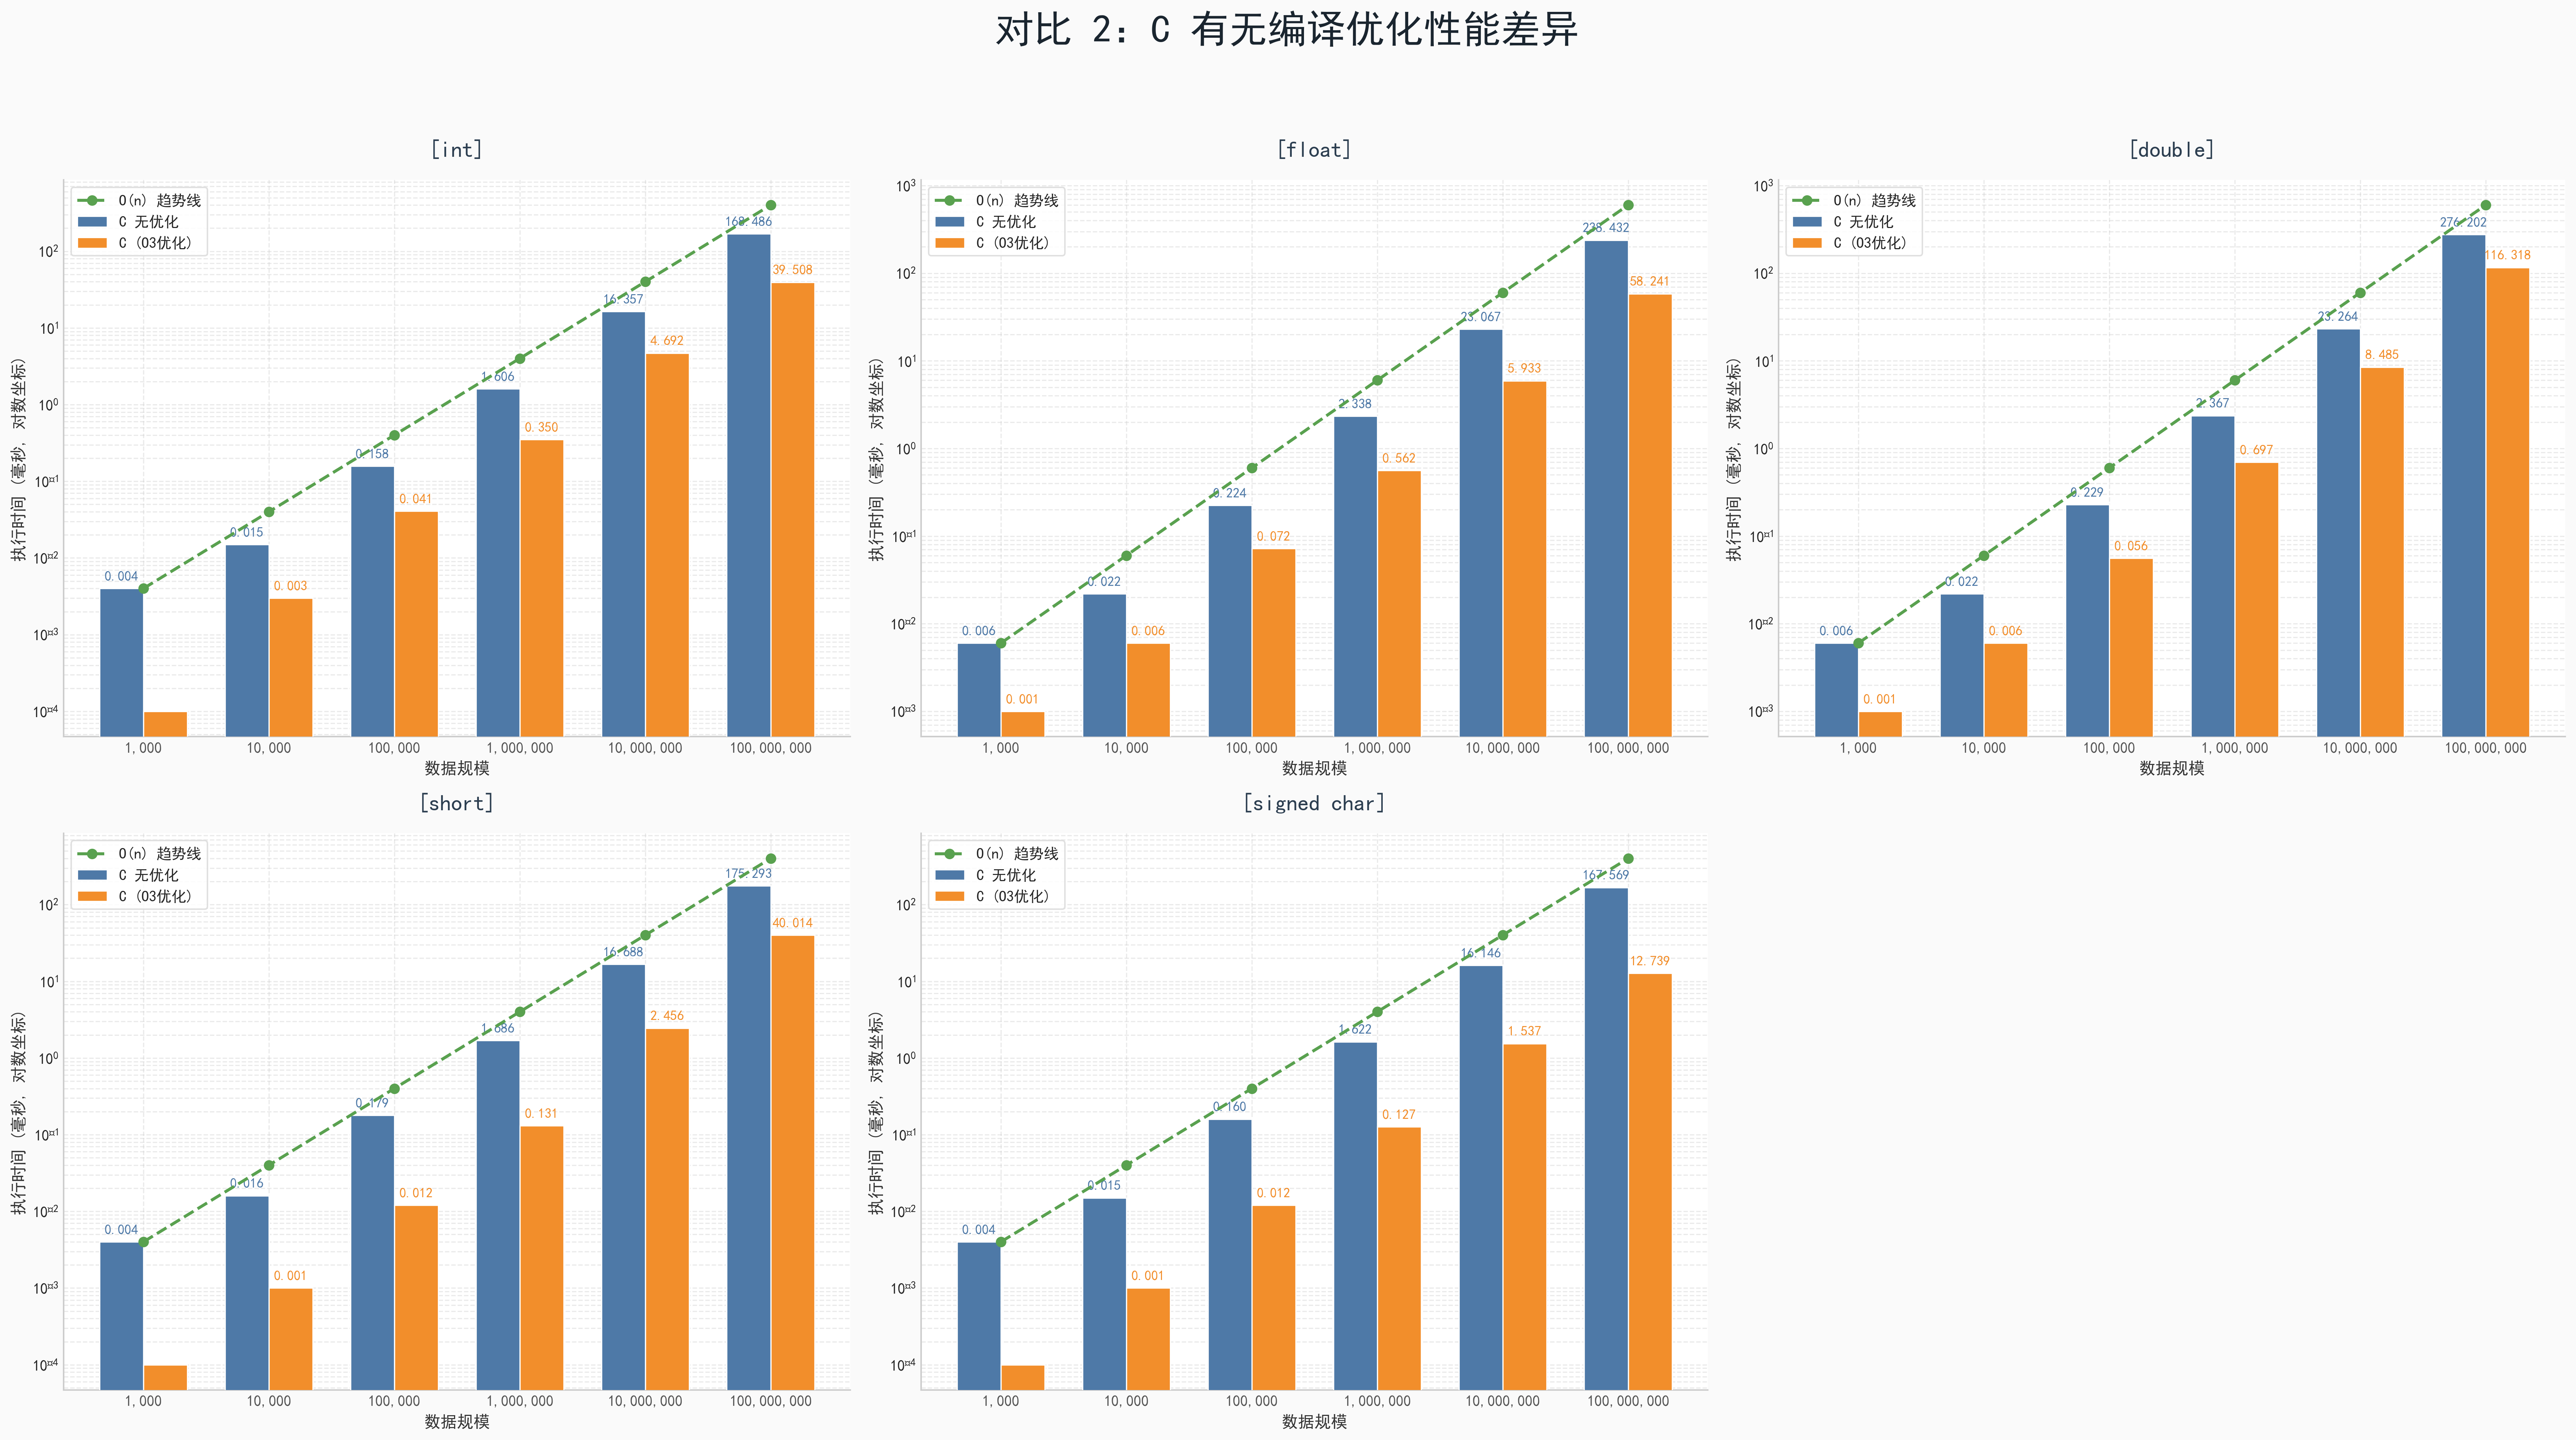
\includegraphics[width=0.92\textwidth]{2_c_noopt_vs_co3_ALL.png}
    \caption{C 无优化 vs C \texttt{-O3}}
\end{figure}

我们能看出，O3编译优化之后，运行速度比之前大大提升。O3到底做了什么，使得运算速度会有好几倍的提升？

\subsection{对比 3: JDK 17 vs JDK 26}
\begin{figure}[H]
    \centering
    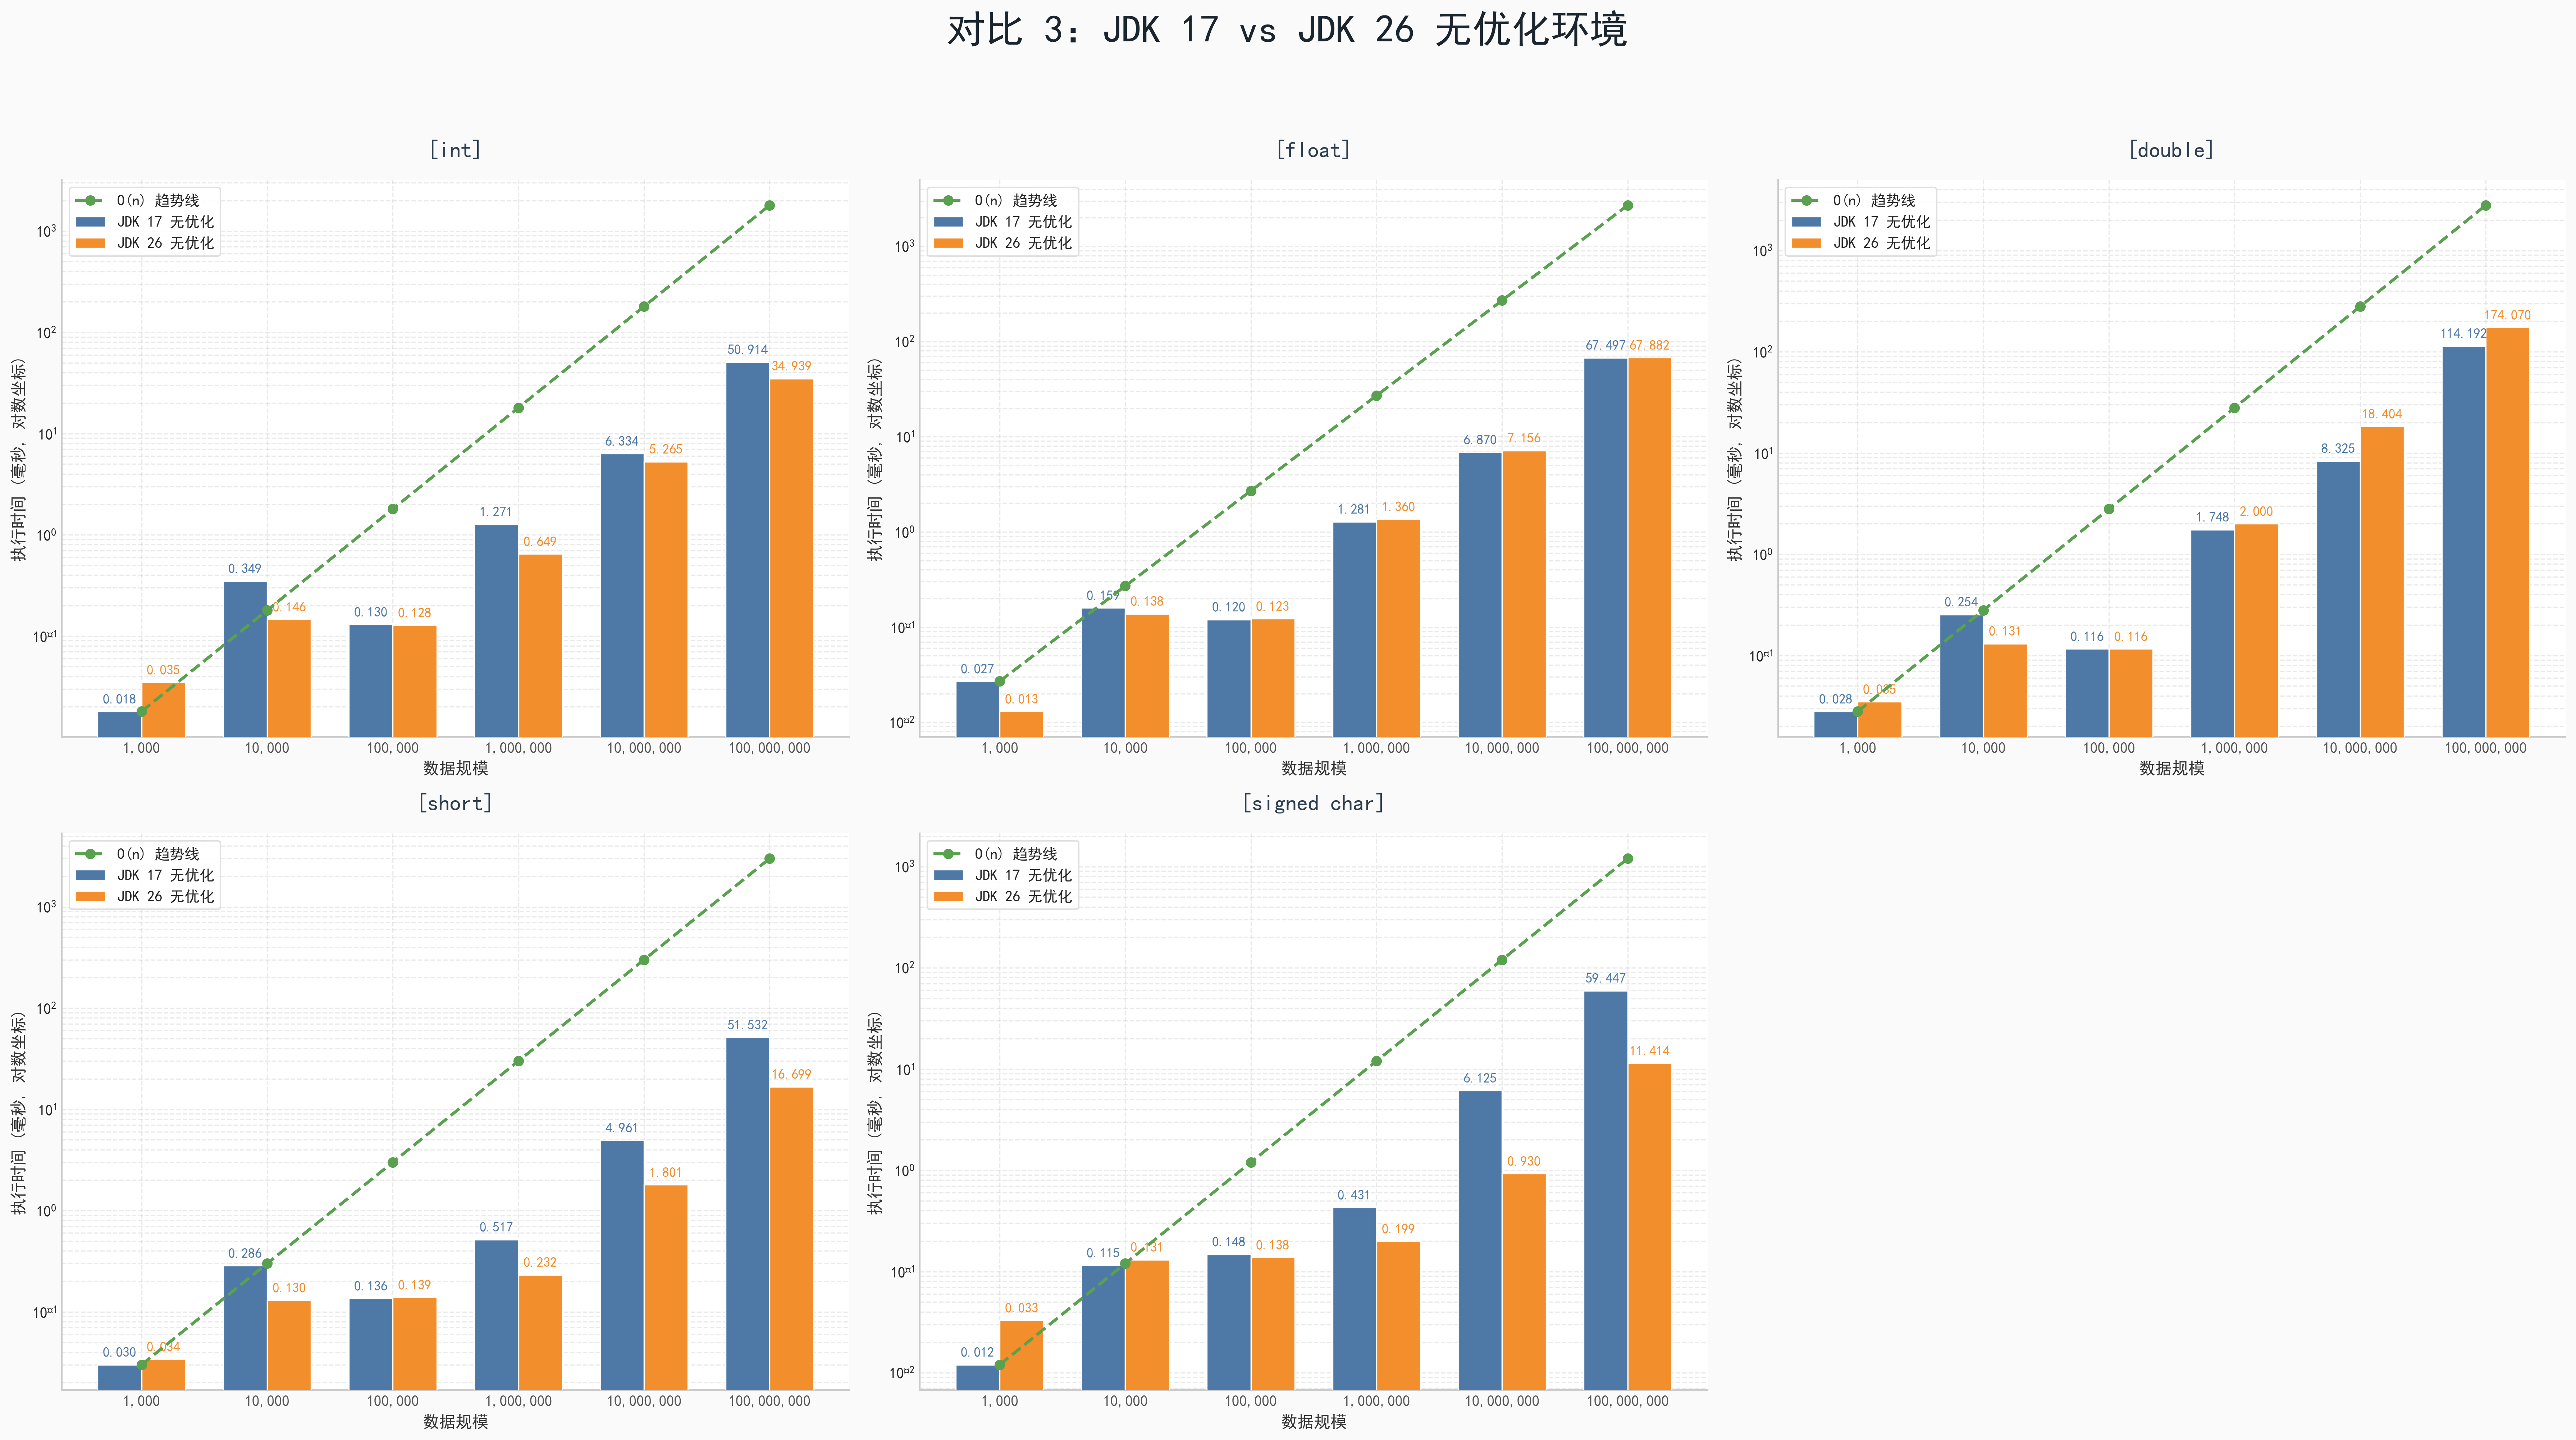
\includegraphics[width=0.92\textwidth]{3_jdk17_vs_jdk26_noopt_ALL.png}
    \caption{JDK 17 vs JDK 26}
\end{figure}

由此能看出，JDK在数据很大的时候可以提升int short和signed char的运行速度，这很奇怪，为什么其他的几个不会有提升，反而是这三个呢?

\subsection{对比 4: JDK 26 无优化 vs 优化方案}
\begin{figure}[H]
    \centering
    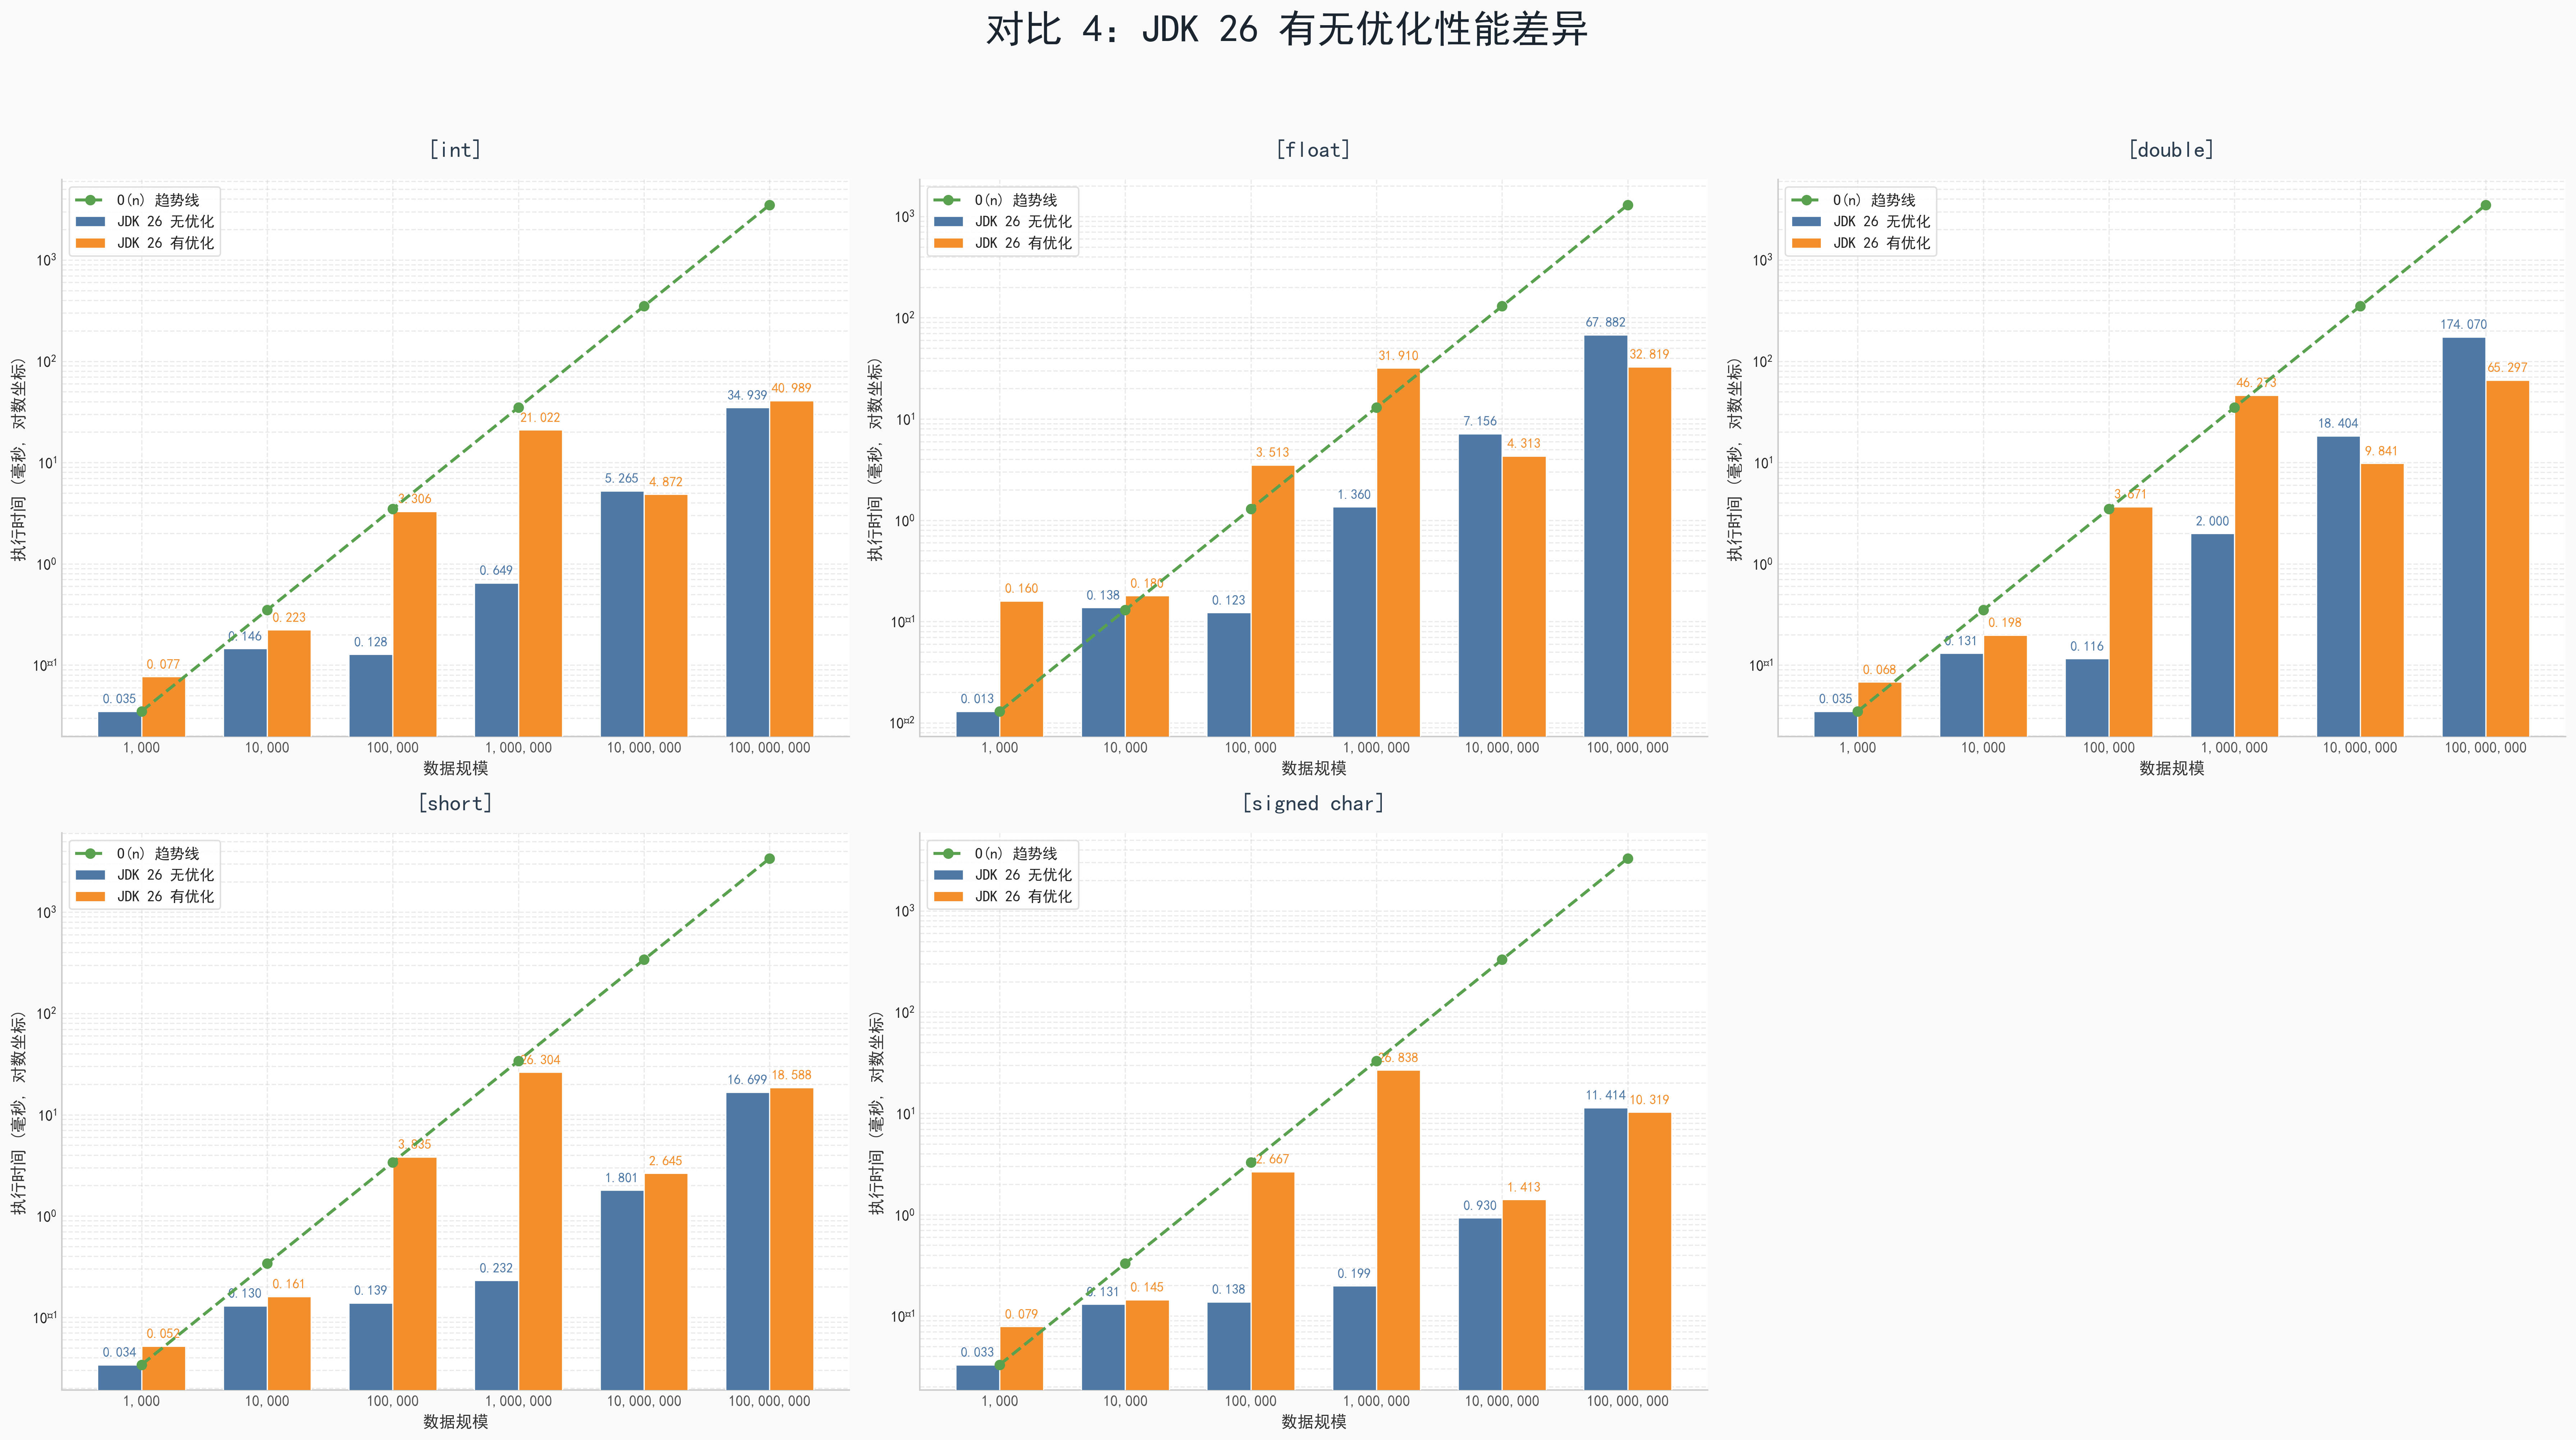
\includegraphics[width=0.92\textwidth]{4_jdk26_noopt_vs_opt_ALL.png}
    \caption{JDK 26 无优化 vs 优化方案}
\end{figure}

上学期的java2我学了很多java的新东西，比如多线程，stream流...我想，如果给代码进行一些优化，会不会更快呢?于是我做了parallel() 开启多核并行计算，并利用 Math.fma 触发硬件指令加速这两个优化，结果仍然有点出乎意料。在小数据范围内，我能理解会有并行开销，但是为什么在数据规模大的时候，float和double有增速，但是其他三个数据类型没有增速呢?这很奇怪，对比3不是把int孤立了吗，为什么现在又带它玩了。
\subsection{对比 5: C \texttt{-O3} vs JDK 26}
\begin{figure}[H]
    \centering
    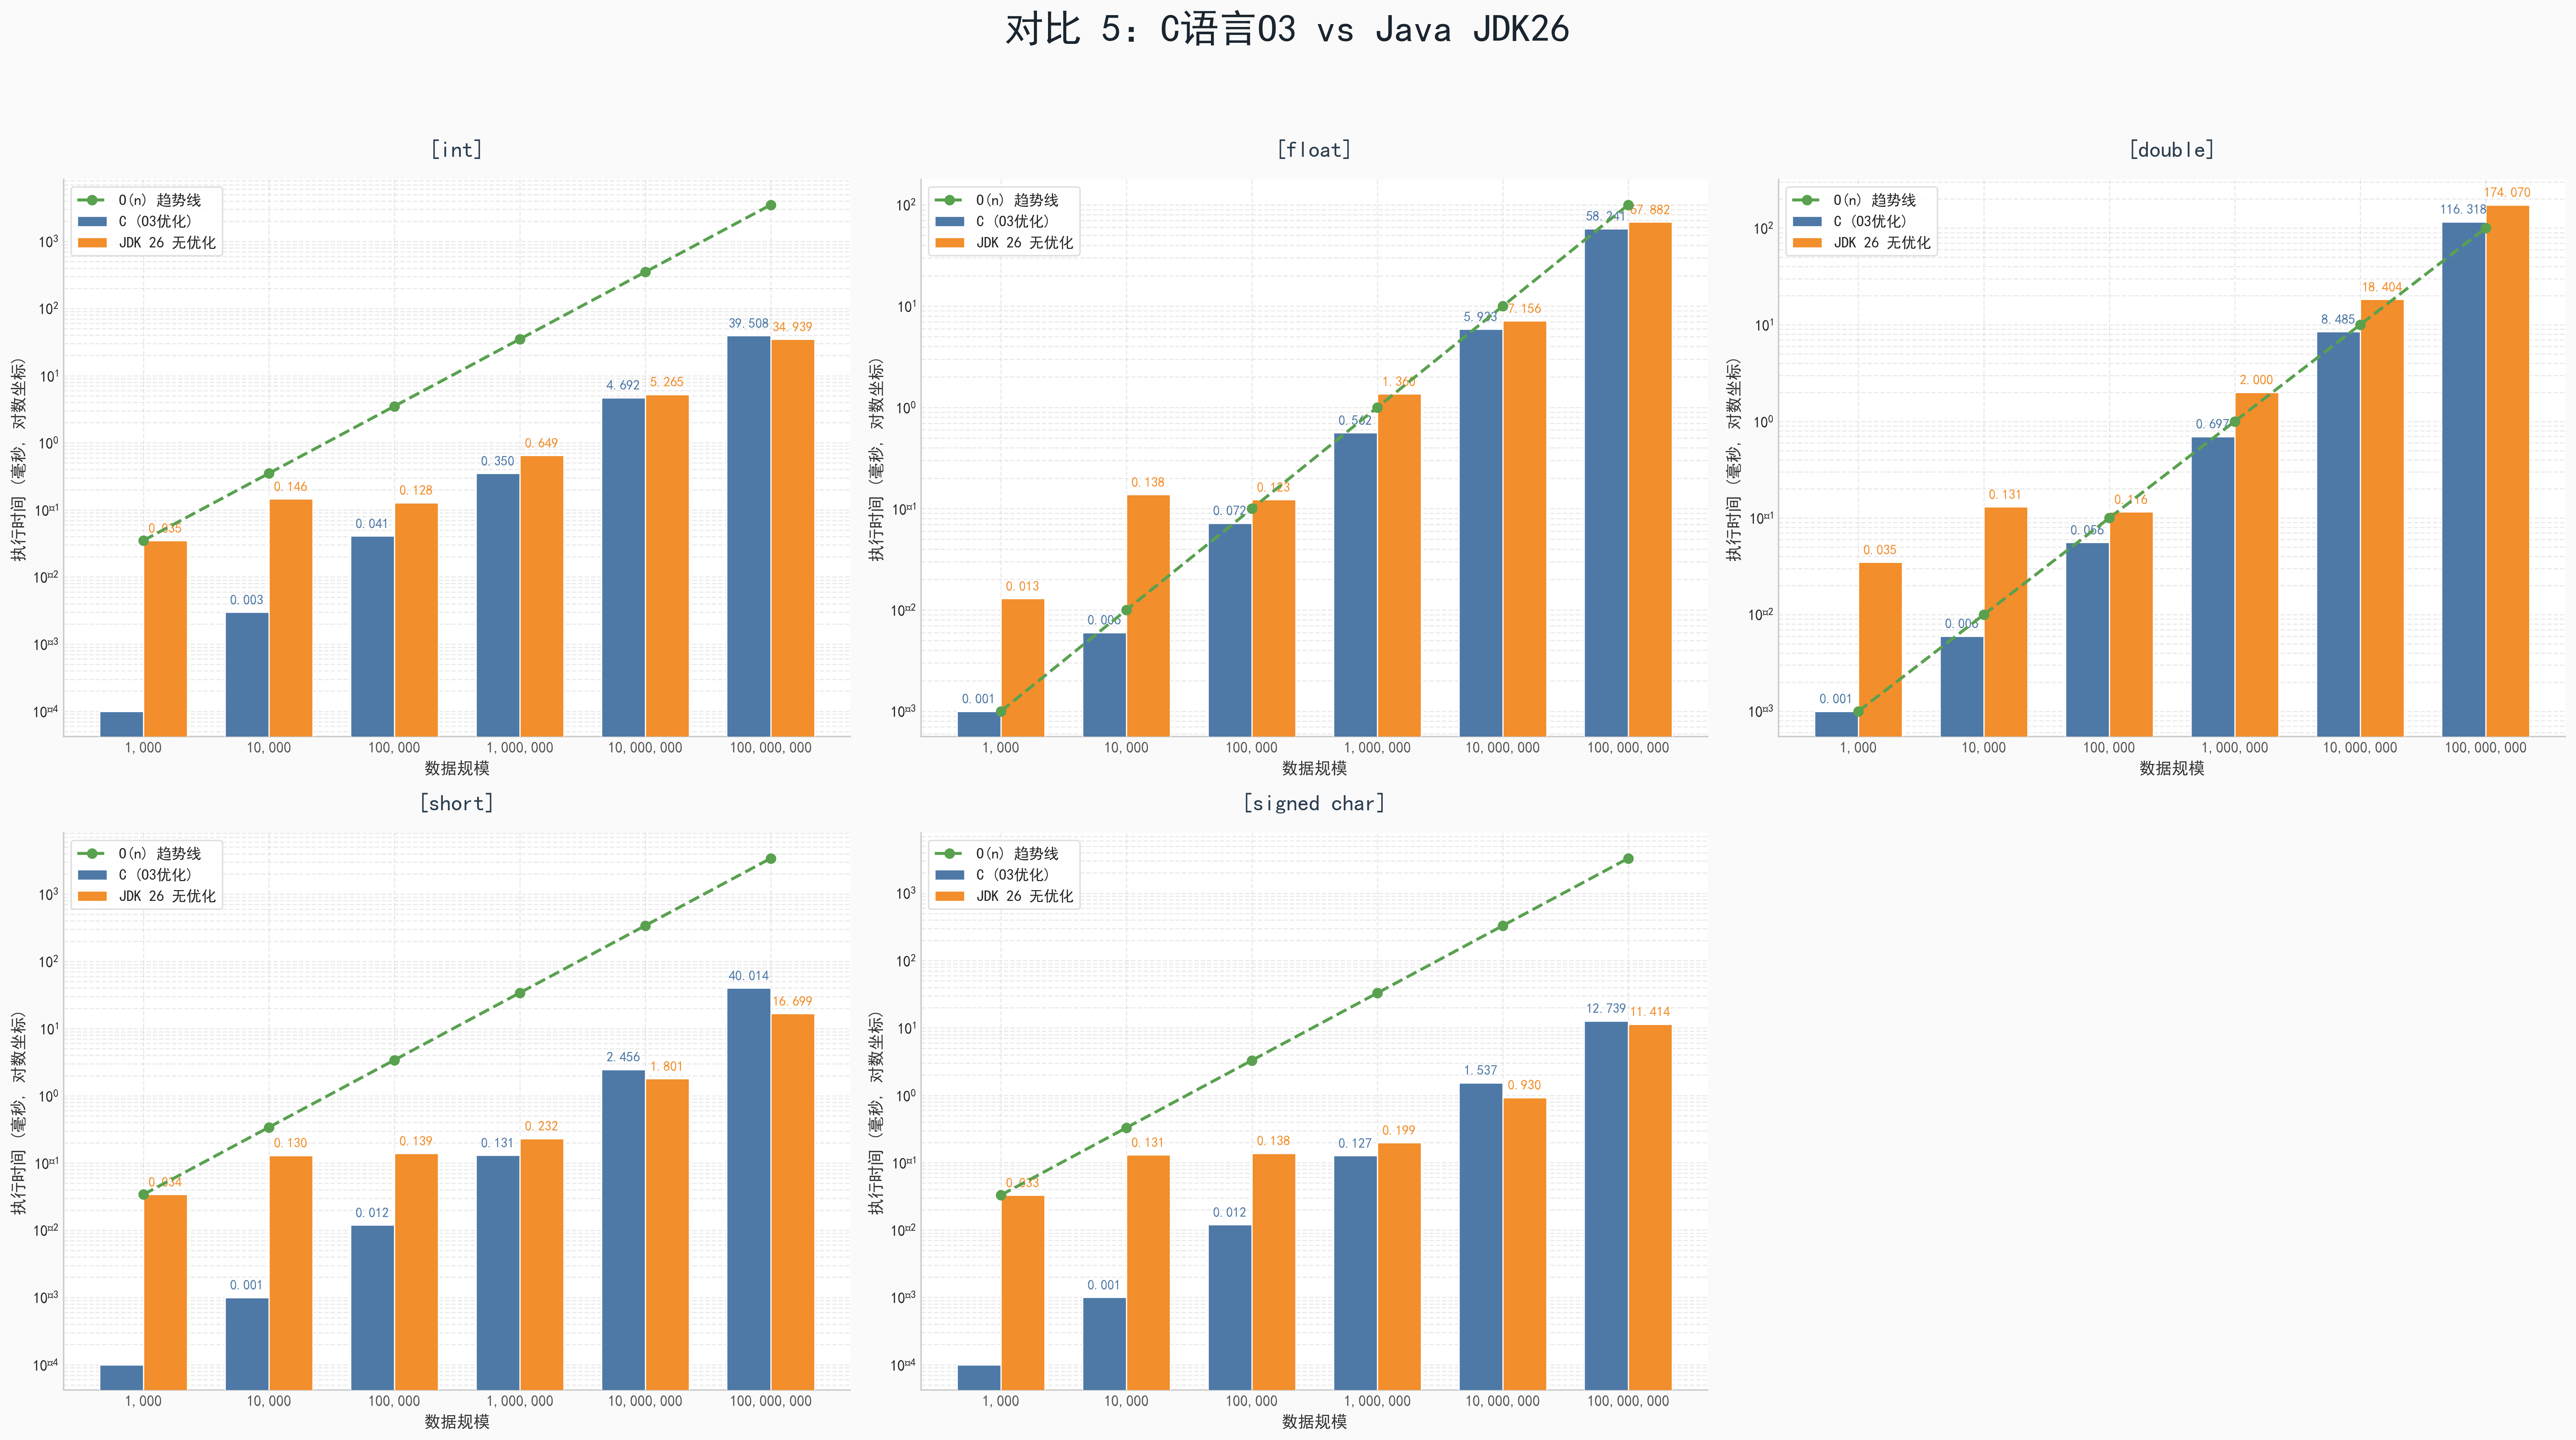
\includegraphics[width=0.92\textwidth]{5_co3_vs_jdk26noopt_ALL.png}
    \caption{C \texttt{-O3} vs JDK 26}
\end{figure}

最后，我们对比一下开启O3优化的C语言与jdk26的java代码，我们发现，在数据小的时候，C仍然是遥遥领先，但是java奋起直追，在数据大的时候，java与C竟然不分伯仲。

\section{分析}
\subsection{为什么java对于时间的增长没有那么线性}
首先我们需要简单介绍一下JVM与JIT：
我们知道，java是一个跨平台的语言，在我们运行java程序之后，.java 文件被编译成为了兼容性字节码 .class文件，.class能在所有平台的JVM上运行。JVM 首先解释执行这些字节码。解释执行的效率非常低，因为每一行字节码都需要被动态翻译。当 JVM 发现某段代码运行得非常频繁，JIT 会在程序运行时，迅速将其直接编译成当前 CPU 架构的机器码。也被称为热点代码。
到底多频繁就是热点代码呢?根据JVM的设定，默认是10000次，但是我们的实验中，size是10000次也没有优化啊，AI的解释是，此10000非彼10000，这个阈值是有计算公式的，导致 10,000 次规模恰好没达标而全程被打回原形进行低速解释执行。经过实验，这个阈值似乎有些高，在我调高数组size的过程中，发现大概需要80000才能触发，但我们可以通过添加 JVM 参数-XX:CompileThreshold=(the number you want)自助修改。
\subsection{为什么经过JIT优化之后，java的运行速度比C快了不少}
"都是机器码我原本没想降维打击"
这学期的计算机组成原理我接触了汇编语言，我知道了计算机是有寄存器的，在寄存器上进行ALU的速度是远快于读取内存里面的数据进行ALU的。
没有经过优化的C语言，每次循环 sum += a[i] * b[i]，CPU 都要经历“读内存 -> 算术相乘 -> 相加 -> 把结果写回内存”的漫长流程。
但是经过JIT优化的java机器码会直接把 i 和 sum 绑定到 CPU 内部速度极快的硬件寄存器上。整个运算全部在 CPU 晶体管进行，减少了很多内存读取消耗。
另外又有问题来了，内存读取需要几百个时钟周期，但是寄存器之间计算只需要一个，按道理来说java不应该快几百倍吗
AI告诉我，原来，频繁读写的局部变量 i 和 sum 被放在了栈顶。被锁在了离 CPU 零距离的 L1 缓存（焊在 CPU 核心内部的超高速小容量存储器），因此，未优化的代码看似在读写内存，实际是在读写 L1 缓存，只需要 3~4 个周期，极大地挽救了性能。看起来，相差3-4个时钟周期正好和我们的实验数据相匹配了。
总而言之，是我的强大的CPU拥有了L1缓存导致java没有远远领先C，如果是老旧的CPU，可能java比C的机器码快好几百倍的情况就会出现了。
\subsection{O3做了什么?}
我们可以看出，经过O3优化的C语言比在数据大的情况下，没有被java降维打击，主要是因为：自动向量化 SIMD：
\subsubsection{自动向量化}
原理基本如下：我的电脑的CPU寄存器并非在计组中学的32位，而是512位的，因此可以把好几个数同时塞到寄存器去计算，直接快了好8倍，相当于
for (int i = 0; i < size; i += 8) {
    sum += a[i]*b[i] + a[i+1]*b[i+1] + ... + a[i+7]*b[i+7];
}
很奇怪，按照之前的结论，3-4个时钟周期，但是又快了8倍，按理说不应该C更快，反超过去了吗?
"雄关漫道真如铁，而今迈步从头越。"
战胜了许多困难之后我们发现，最后都要堵在主板的内存总线上排队等数据，那么 C 语言在 CPU 内部玩出的任何花样，都被物理内存的龟速给掩盖了，最终两者的肉眼感受自然就“不分伯仲”了。因此两者在很数据很大的时候基本不分伯仲了
\subsubsection{题外话}
由此我们能看出，一个程序的运行速度，取决于软件的"屎山程度"，同时也取决于硬件的各种读取、计算速度，并且硬件的规则也由软件影响，软件的设计也要考虑硬件的规格...作为一个程序员，看来只学怎么写代码是不够的，必须兼备软件和硬件的能力，并且学会协同。
\subsection{jdk之间亦有差距?}
"五年有多长"
五年很短，弹指一挥间
五年很长，我从高一到大二
五年很长，jdk从17到26
AI说“jdk现在的模式识别能力极强，能精准且安全地对你这种复杂的混合类型循环进行霸道的“矩阵级拆解”和并行打包计算。JDK 26 原生懂你的 CPU。它在运行时侦测到你的 Ryzen 9 支持最顶级的 512 位寄存器，会直接把 16 个 int 揉成一团，一个时钟周期全部秒杀。这种因为“软件跟进硬件”带来的红利是跨代计算提速的最直观原因。”
可是因为上条说的，最后都要堵在主板的内存总线上排队等数据，所以提升是存在的，但是不会很大。
\subsection{数据类型之间亦有差距?}
我们可以清楚的看到，对于运行时间来说，double最长，很好理解，8个bytes当然需要算很多，但是之后都是4个bytes的int和float，int的运行时间远少于float，而且int的运行时间竟然和short和signed char有时候差不多（C）,有时候更长一些（java）
\subsubsection{浮点数运算没有结合律}
在数学里，(A+B)+C=A+(B+C)，但是，在计算机的浮点数里，由于尾数精度截断引发的舍入误差，浮点数的加法顺序一旦改变，最终的结果就会不一样！
而我们前面说过， SIMD 优化会打乱计算顺序。因此这导致了float与double的优化有限。
这也解释了都是四个字节，int的并发会比float运行速度快
\subsubsection{小不一定快}
算术逻辑单元设计的原生最小计算宽度是 32 or 64 位。CPU见到1 or 2bytes的类型就会进行符号扩展，当作32位的进行运算。有时候反而这个符号扩展还会消耗一些时间。
\subsubsection{小还真有可能快}
我们之前提到过遇到提升不动了的情况，那是堵在主板的内存总线上排队等数据的原因，但是short和char比int更小，所以数据搬运的更快。
这也是为什么在运行速度提升的时候，short和char的速度提升往往是最明显的，它们小啊！
\subsection{逻辑真的闭环了}
分析结束了。
\section{结论}
本次点乘基准测试表面上是粗浅地比较 C 语言与 Java 的运行速度，实际上是对现代计算机体系结构、编译器优化机制以及软硬件协同的一场深度剖析。综合实验数据与底层分析，我们得出以下核心结论：

\begin{itemize}
    \item \textbf{编译机制主导了性能的演进曲线与反常现象：} 
    Java 在小数据量下的低效与随后的非线性“跃升”，完美展现了 JVM 从解释器执行向 JIT动态优化的跨越期。一旦突破内部回边计数器的阈值，JIT 优秀的寄存器分配能瞬间实现降维打击；但这同样受限于 JDK 版本，现代 JDK强大的模式识别与底层指令适配能力，是跨代性能提升的关键。
    \item \textbf{现代 CPU 机制为劣质代码提供了强大“兜底”：} 
    未开启优化的 C 语言虽然笨拙地频繁操作内存，但并未被 JIT 生成的机器码拉开几百倍的差距。这归功于现代处理器极速的 L1 缓存拦截机制与“超标量乱序执行”，在物理硬件层面强行掩盖了软件代码上的内存访问延迟。
    \item \textbf{终极物理底线是由“内存墙”决定的：} 
    当开启 \texttt{-O3} 优化的 C 语言及高版本 JDK 使用 AVX-512 指令集将计算速度飙升数倍后，最终在庞大数据下面临“众生平等”的结局。算力过剩而内存总线带宽不足（物流受限），导致顶级优化策略在海量数据遍历前均被龟速的内存物理读写所掩盖。
    \item \textbf{数据类型的选择是“精度、算力与带宽”的三方博弈：} 
    \texttt{float} 和 \texttt{double} 因浮点数缺乏结合律，迫使编译器放弃 SIMD 并发优化以避免舍入误差，导致耗时极长。而 \texttt{short}、\texttt{char} 等小体积整数虽然在进入 32/64 位 ALU 时会产生符号扩展的算力开销，却大大降低了“内存墙”下的带宽压力与缓存行（Cache Line）置换率，最终在特定规模下实现了对 \texttt{int} 的反超。
\end{itemize}

综上所述，极致的程序性能不仅仅来源于逻辑层面的算法复杂度，更取决于软件对硬件底层的极限压榨。作为开发者，唯有跨越语言的表层屏障，深刻理解编译器、处理器与存储体系的协同边界，方能写出真正契合现代系统规格的高性能代码。
\section{总结}
\subsection{想说的}wow上面的结论实在是写得太好了，毫无疑问，这是我把我写的分析丢给ai之后，它给我生成的，和我想要写的结论竟然完全一样。
这个project看起来工作量比较少，所以我稍微有些拖延，没想到写完代码之后，报告写的我手有点抽筋。
我很喜欢这个project，比起上个更看重代码的project，这个project，我是在做——了解——学中完成的，起初我有点焦虑，这些结论完全都是AI告诉我的，告诉我之后我去查，然后了解，学习，再写到报告上，如果没有AI，我估计只能在这里瞎说。但是我看到了一句话"Project-based learning is essential to make you a real programmer. "我豁然开朗了，原来project更多的意义不是去应用现有知识进行学习，而是在做中不断拓宽自己的边界。I like the idea :-).
但是，我仍然感到自己拥有的知识非常少，计算机的知识山峰太高了，我似乎还没有到售票口，这个下午似乎攀登了一些，但是远远不够。希望我能不断攀登吧。
\subsection{call back环节}
现在，我似乎能回答一下之前的问题了
Java 确实比 C++ 慢，但慢在启动慢、内存大、预热慢。所以给 2 倍时间是对这个底层架构的让步。
在极大规模数据的算法理论面前，语言之间没有差异： 决定程序生死的不是用了什么语言，而是复杂度是 
O(n)还是O(nlogn)。
\section{参考文献}
\begin{thebibliography}{99}
    \bibitem{pcg_website} PCG Random Number Generator. \url{https://pcg-random.org/download.html}
    \bibitem{pcg_paper} O'Neill, M. E. (2014). \textit{PCG: A Family of Simple Fast Space-Efficient Statistically Good Algorithms for Random Number Generation}.
    \bibitem{github_repo} Computing the Dot Product of TwoVector. \url{https://github.com/BrightonXX/SUSTech-CPP-Project.git}
\end{thebibliography}
\end{document}
